% -- LaTeX rewrite of main.typ, using the OUP template and matching the structure and content --

\documentclass[unnumsec,webpdf,contemporary,large]{oup-authoring-template}
\usepackage{booktabs}
\usepackage{placeins}
\usepackage{float}

\theoremstyle{thmstyleone}%
\newtheorem{theorem}{Theorem}%
\newtheorem{proposition}[theorem]{Proposition}%
\theoremstyle{thmstyletwo}%
\newtheorem{example}{Example}%
\newtheorem{remark}{Remark}%
\theoremstyle{thmstylethree}%
\newtheorem{definition}{Definition}

\begin{document}

\journaltitle{Oxford University Press.}
\copyrightyear{2025}
\appnotes{Paper}

\firstpage{1}
\setlength{\parindent}{0pt}
\setlength{\parskip}{0em}

\title[Short Article Title]{Assessing the Reliability of AlphaFold3 Predictions for Protein-Ligand Affinity Prediction via Sfcnn}

\author[1]{Guo Yu}
\author[1]{Yiming Wu}
\author[1]{Yiyang Tan}

\authormark{Guo Yu et al.}

\address[1]{\orgdiv{School of Information Science and Technology}, 
\orgname{ShanghaiTech University}, 
\orgaddress{\street{393 Middle Huaxia Road}, \postcode{201210}, \state{Shanghai}, \country{China}}}

\abstract{
This study systematically evaluates the reliability of AlphaFold3 (AF3)-predicted protein structures for protein-ligand affinity (PLA) prediction tasks. The Sfcnn model, a 3D convolutional neural network (CNN) for PLA prediction, was reproduced using PyTorch. Model performance was validated on the PDBbind v2019 refined set for training and the CASF-2016 core set for testing. Subsequently, AF3-derived protein structures from the CASF-2016 core set were assessed and compared to experimentally determined structures using Sfcnn scores, to determine the suitability of AF3 predictions in PLA applications.
}
\keywords{AlphaFold3, protein-ligand affinity, CNN scoring function, CASF-2016}

\maketitle

\section{Introduction}

\subsection{Sfcnn Overview}
\vspace{0.5em}
Sfcnn is a 3D convolutional neural network-based scoring function introduced by Wang et al.~\cite{Sfcnn} in 2022, designed to provide accurate and reliable predictions of binding affinities for protein-ligand complexes.

\section{Methods}

\subsection{Datasets}
\vspace{0.5em}
The Sfcnn network was trained using protein-ligand complexes from the PDBbind v2019 refined set, which includes experimentally determined binding affinities (pKa values). The model was evaluated on the CASF-2016~\cite{su2018comparative} core set, comprising 285 protein-ligand complexes. To prevent data leakage, 266 overlapping protein complexes between the training and test sets were excluded, resulting in 4,852 unique training complexes.

\subsection{Data Augmentation}
\vspace{0.5em}
To increase the effective size of the training set, each protein-ligand complex was randomly rotated nine times using random rotation matrices, yielding ten variants per complex. All variants share the same PLA score, resulting in a total of 48,520 training samples.

\subsection{Featurization}
\vspace{0.5em}
Protein-ligand complexes are represented as 3D grids of size $20 \times 20 \times 20$, with each grid cell encoded as a one-hot vector of length 28. This vector comprises 14 protein atom types\footnote{\url{https://bmcbioinformatics.biomedcentral.com/articles/10.1186/s12859-022-04762-3}} and 14 ligand atom types. The resulting training tensor has shape $(48520, 20, 20, 20, 28)$.

\begin{figure}[H]
    \centering
    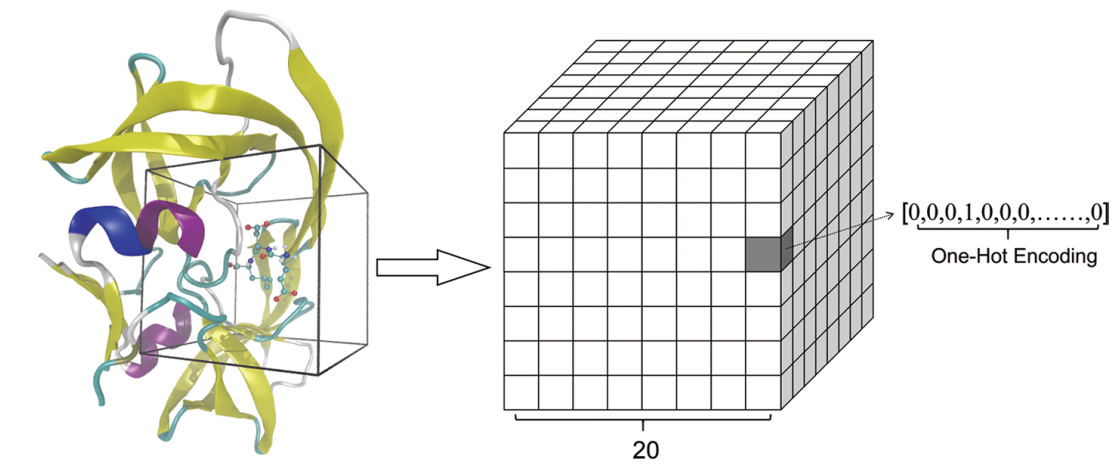
\includegraphics[width=0.5\textwidth]{images/one_hot.png}
    \caption{Featurization of protein-ligand complexes. Example shown: PDB ID 1a30. Default resolution is $20\times20\times20$ with 28 atomic categories.}
    \label{fig:onehot}
\end{figure}

\section{Network Architecture}

The original Sfcnn publication describes four network architectures and three featurization strategies. The architecture depicted in Figure~\ref{fig:CNN}, combined with the aforementioned featurization, achieved optimal validation performance.

\begin{figure}[H]
    \centering
    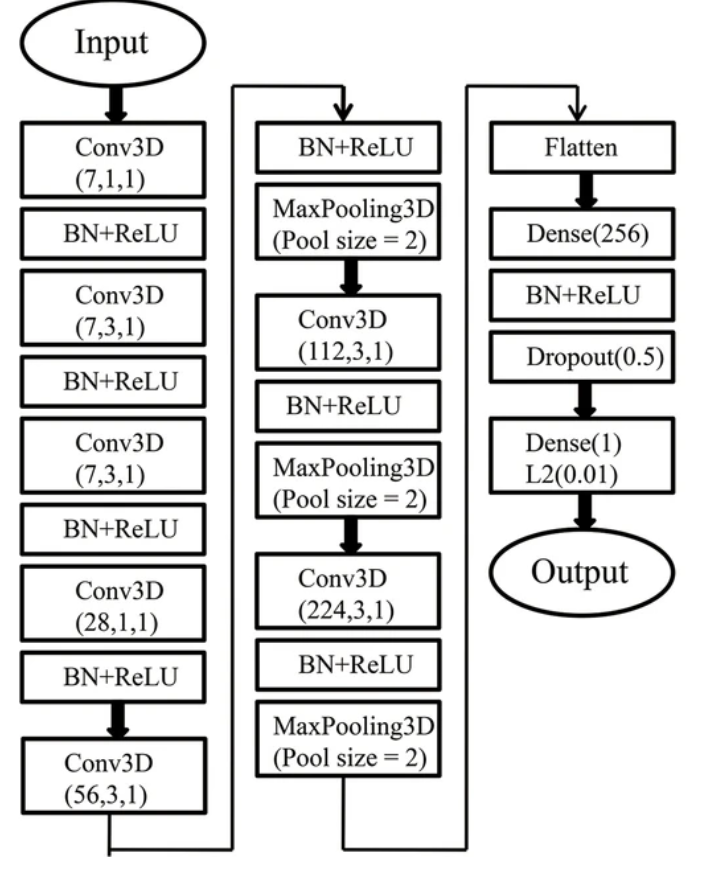
\includegraphics[width=0.35\textwidth]{images/CNN.png}
    \caption{Final CNN architecture for the Sfcnn network.}
    \label{fig:CNN}
\end{figure}

This architecture employs 3D convolutional layers with batch normalization and ReLU activation. L2 regularization is applied to the output layer to mitigate overfitting and enhance generalization.

\section{Reproduction Study}

\subsection{Dataset and Featurization}
\vspace{0.5em}
The reproduction pipeline utilizes the same datasets and featurization approach, yielding a training tensor of shape $(48520, 20, 20, 20, 28)$ and a test tensor of shape $(285, 20, 20, 20, 28)$.

\subsection{Data Storage}
\vspace{0.5em}
The original Sfcnn implementation stored data as concatenated arrays in a single \texttt{.pkl} (pickle) file, requiring all data to reside in memory, which is impractical for extremely large datasets. The format of \texttt{.h5} (HDF5) via \texttt{h5py} is adopted for incremental writing and efficient storage. The resulting training grid occupies 40.1 GiB.

\subsection{Network Implementation}
\vspace{0.5em}
The PyTorch implementation closely mirrors the original TensorFlow version, with two key differences:
\begin{enumerate}
    \item Due to PyTorch's \texttt{Conv3D} API, input tensors are permuted to shape (batch\_size, 28, 20, 20, 20).
    \item PyTorch lacks a direct L2 regularization API; instead, weight decay is applied to the final fully connected layer to approximate this effect.
\end{enumerate}

\subsection{Training Procedure}
\vspace{0.5em}
Training and validation sets are partitioned as in the original study, with the validation set comprising indices 41,000 to 48,520. The resulting splits are: training $(41,000, 20, 20, 20, 28)$, validation $(7,520, 20, 20, 20, 28)$, and test $(285, 20, 20, 20, 28)$, corresponding to a ratio of 84.00\% : 15.42\% : 0.58\%. 
Note that the original hyperparameters did not yield convergence in our PyTorch experiments, both hyperparameters are summarized in the the following table.

\begin{table}[H]
\centering
\caption{Original and Reproduced Hyperparameters}
\label{tab:hyperparams}
\begin{tabular}{lcc}
\toprule
Parameter & Original & Reproduced \\
\midrule
Learning rate & 0.004 & 0.0015 \\
Batch size & 64 & 32 \\
Dropout rate & 0.5 & 0.15 \\
L2 regularization / FC weight decay & 0.01 & 0.01 \\
Epochs & 200 & 200 \\
\bottomrule
\end{tabular}
\end{table}

\subsection{Reproduced Results}

\subsection{Evaluation Metrics}
\vspace{0.5em}
Sfcnn performance is evaluated using the following metrics:

\begin{align*}
\mathrm{RMSE} &= \sqrt{\frac{1}{N} \sum_{i=1}^{N} (y_{\text{predict}} - y_{\text{true}})^2} \\
\mathrm{MAE} &= \frac{1}{N} \sum_{i=1}^{N} |y_{\text{predict}} - y_{\text{true}}| \\
\mathrm{SD} &= \sqrt{\frac{1}{N-1} \sum_{i=1}^{N} ((a y_{\text{predict}} + b) - y_{\text{true}})^2} \\
\mathrm{R} &= \frac{\mathbb{E}[(y_{\text{predict}} - \mu_{y_{\text{predict}}})(y_{\text{true}} - \mu_{y_{\text{true}}})]}{\sigma_{y_{\text{predict}}} \sigma_{y_{\text{true}}}}
\end{align*}

where $a$ and $b$ are the slope and intercept of the linear regression between predicted and measured values, $\mathbb{E}[\cdot]$ denotes expectation, and $\mu$ and $\sigma$ represent means and standard deviations, respectively.

\begin{table}[H]
\centering
\caption{Performance Metrics on CASF-2016 Core Set}
\label{tab:metrics}
\begin{tabular}{lcc}
\toprule
Metric & Reproduced Sfcnn & Original Sfcnn \\
\midrule
Pearson R & 0.7286 & 0.7928 \\
RMSE & 1.5481 & 1.3263 \\
MAE & 1.2579 & 1.0277 \\
SD & 1.4892 & 1.3252 \\
\bottomrule
\end{tabular}
\end{table}

Although the original Sfcnn reports superior metrics, its training process did not converge in the reproduction, raising concerns regarding the reproducibility of the reported performance. Due to the lack of access to the original training data and the absence of author response to data requests on GitHub\footnote{\url{https://github.com/bioinfocqupt/Sfcnn/issues/1}}, the original training process is deemed irreproducible.

The training, validation, and testing results for the four metrics are presented in Figure~\ref{fig:ReproducedPlot} and Figure~\ref{fig:OriginalPlot}.

\begin{figure}[H]
    \centering
    \begin{minipage}{0.5\textwidth}
        \centering
        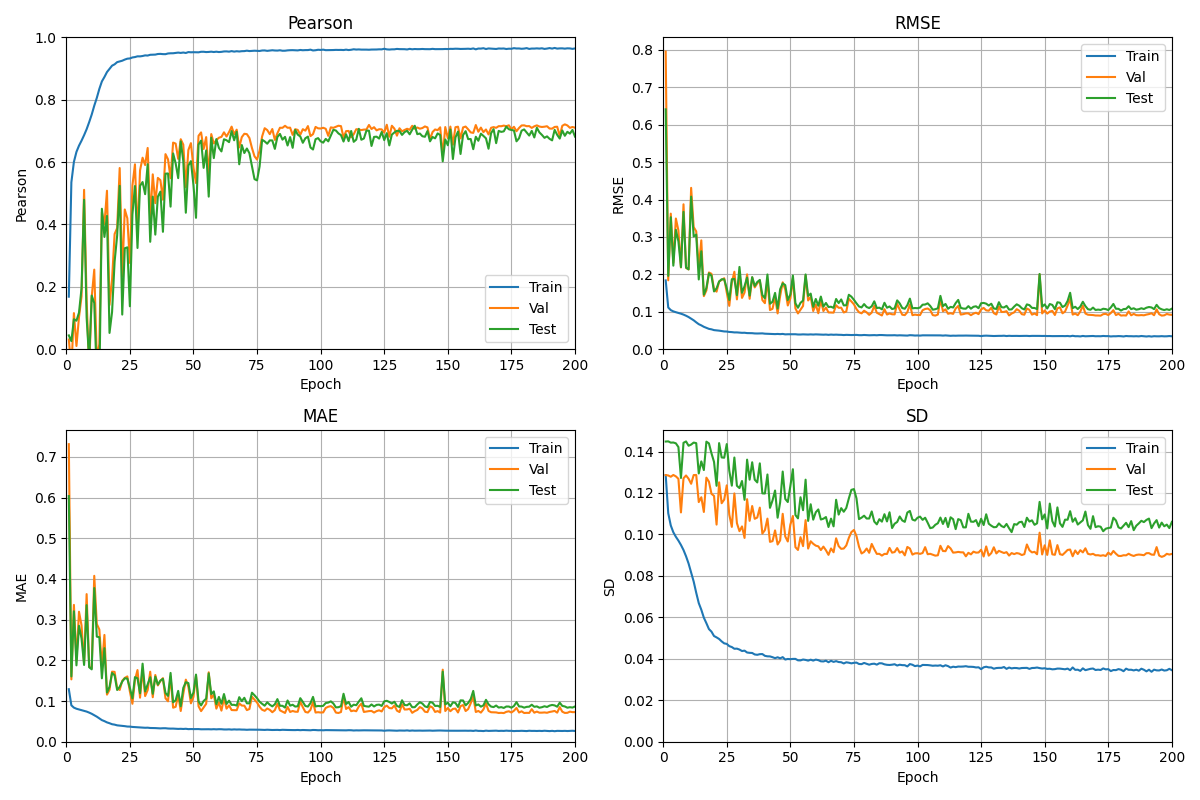
\includegraphics[width=\textwidth]{images/normal_converge.png}
        \caption{Training curve for reproduced hyperparameters.}
        \label{fig:ReproducedPlot}
    \end{minipage}\hfill
    \begin{minipage}{0.5\textwidth}
        \centering
        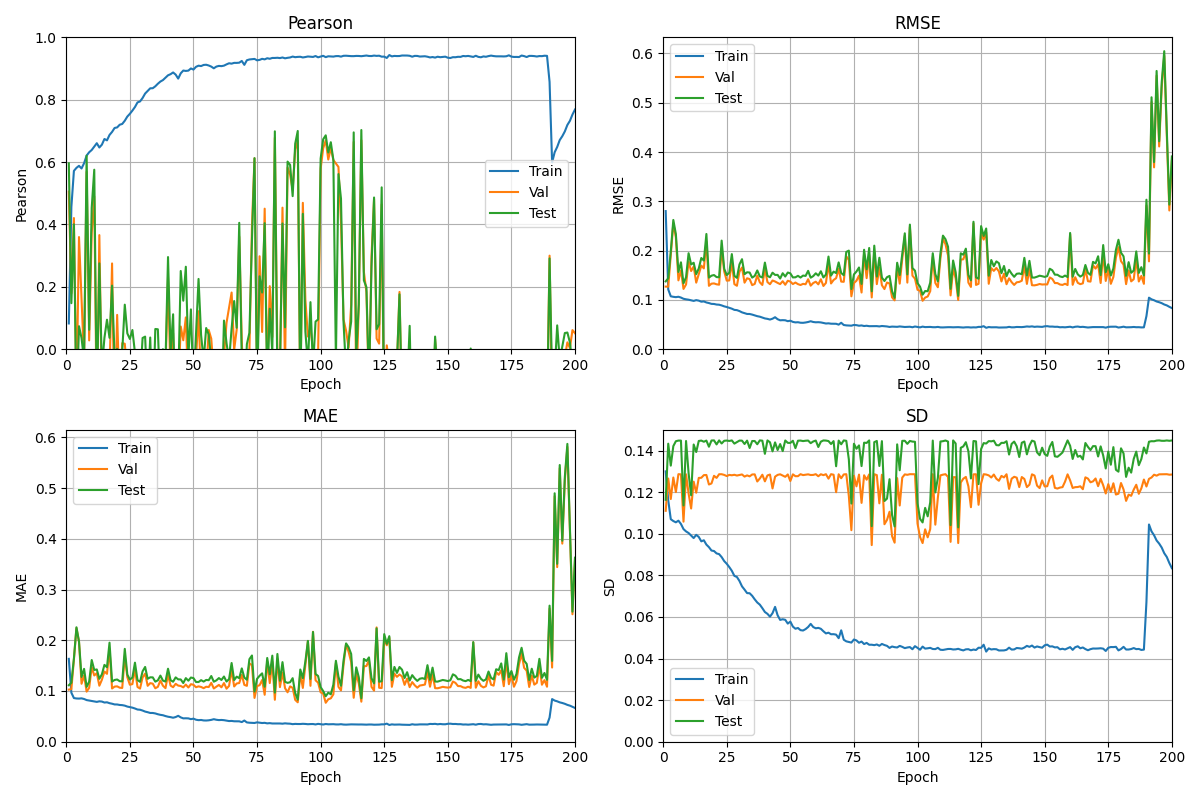
\includegraphics[width=\textwidth]{images/origin_param.png}
        \caption{Training curve for original hyperparameters.}
        \label{fig:OriginalPlot}
    \end{minipage}
\end{figure}

\vspace{-2.5em}
Since the original hyperparameters significantly deviate from the 
norm and did not reach proper comvergence,
the reproducted results are 
considered the baseline for subsequent AF3 result assessment.

\vspace{-1em}
\section{AlphaFold3 Structure Assessment}

\subsection{Dataset}
The assessment utilizes the CASF-2016 core set, excluding six proteins with structural complexity beyond AlphaFold3's predictive capacity, resulting in 279 proteins. Proteins with more than five isomorphic or heterogeneous chains were excluded, as detailed in Table~\ref{tab:complex}.
\vspace{-1em}
\begin{table}[H]
\centering
\caption{Excluded Complex Protein Structures}
\label{tab:complex}
\begin{tabular}{lc}
\toprule
PDB ID & Number of Chains \\
\midrule
2xb8 & 12 \\
2ymd & 10 \\
3n76 & 12 \\
3n7a & 12 \\
3n86 & 12 \\
4ciw & 12 \\
\bottomrule
\end{tabular}
\end{table}

\subsection{Workflow}
\vspace{0.5em}
\paragraph{Structure Generation}
Protein structures were generated using the \textit{Chai-1 online server}\footnote{\url{https://lab.chaidiscovery.com/dashboard}}. The AlphaFold3 online server\footnote{\url{https://alphafoldserver.com/}} was not used due to its inability to accept specific ligand SMILES codes. The MSA (Multiple Sequence Alignment) option was enabled with the MMseqs2 algorithm for all generations.

\paragraph{Docking and File Handling}
Server outputs were downloaded as zip archives containing multiple ranked structures and associated metrics. The top-ranked structure (\texttt{pred.rank\_0.cif}) was selected for analysis. To avoid conversion errors between file formats (.cif, .pdb, .mol2), structures were parsed directly using the \texttt{MMCIFParser} from Bio.PDB, followed by featurization and grid mapping.

Atoms or isotopes not included in the 14 predefined atom types are categorized as \texttt{other}.

\paragraph{Scoring}
Predicted structures were scored using the reproduced Sfcnn network, loaded with pre-trained weights (Pearson R = 0.728). Detailed analysis of PLA results and metrics is provided in the subsequent section.

\subsection{Result Analysis}
\vspace{0.5em}
[Detailed analysis of the results should be inserted here.]

\section{Conclusion}
This study presents a systematic evaluation of AlphaFold3-predicted protein structures for protein-ligand affinity prediction using a reproduced Sfcnn model. The findings highlight the importance of reproducibility in deep learning models for structural biology and demonstrate the current capabilities and limitations of AF3 in the context of PLA prediction. [Further conclusions and implications should be added here.]

\section{External Libraries}

\begin{itemize}
    \item \textbf{PyTorch}: Custom neural network implementation.
    \item \textbf{Pandas}: Data storage and analysis.
    \item \textbf{Numpy}: Data processing and manipulation.
    \item \textbf{Matplotlib}: Visualization of training loss curves.
\end{itemize}

\section{Author Contributions}
G.Y., L.T., and J.C. conceived, conducted, and analyzed the experiments, and contributed to manuscript preparation and review.

\section{Acknowledgments}
The authors thank the anonymous reviewers for their valuable feedback. This work was supported in part by the National Science Foundation (NSF: \#1636933 and \#1920920).

\bibliographystyle{plain}
\bibliography{reference}

\end{document}